\definecolor{srblue}{RGB}{196,124,73}
\definecolor{srgreenfill}{RGB}{255,244,232}
\definecolor{srgreendraw}{RGB}{198,132,76}
\definecolor{srorangefill}{RGB}{255,236,214}
\definecolor{srorangedraw}{RGB}{221,132,59}
\definecolor{srgrayfill}{RGB}{252,245,238}
\definecolor{srgraydraw}{RGB}{141,118,100}
\definecolor{srhwfill}{RGB}{245,233,221}
\definecolor{srtext}{RGB}{34,38,45}

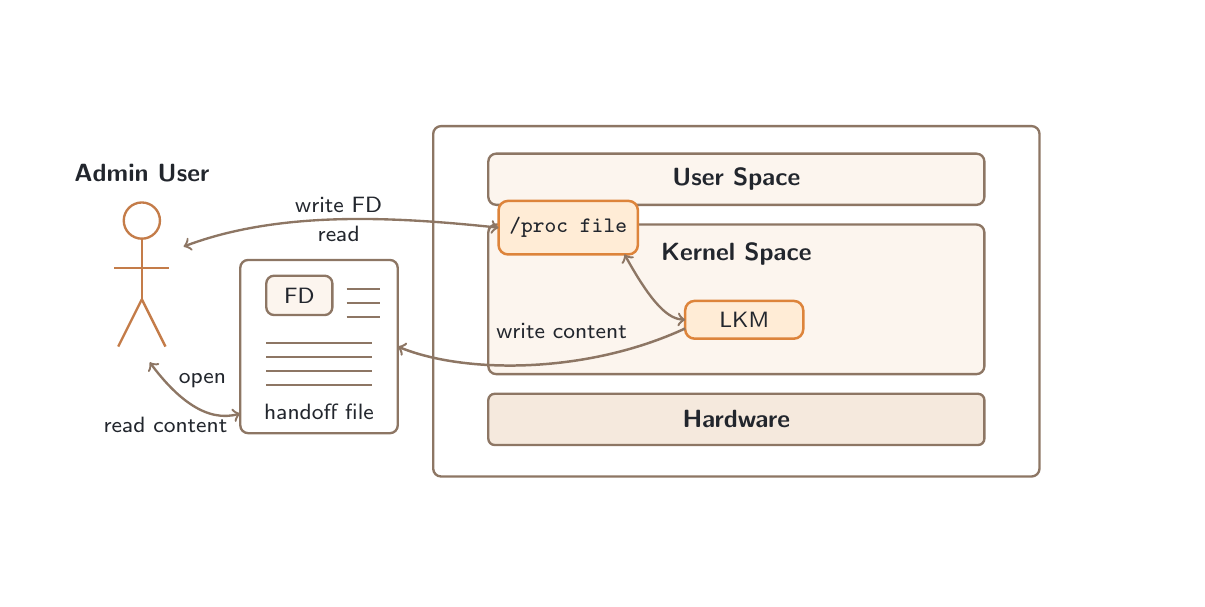
\begin{tikzpicture}[
  x=1cm,
  y=1cm,
  every node/.style={inner sep=0pt, outer sep=0pt},
  label/.style={font=\sffamily\fontsize{8}{8.6}\selectfont, text=srtext, align=center},
  title/.style={font=\sffamily\bfseries\fontsize{9}{9.6}\selectfont, text=srtext, align=center},
  block/.style={draw=srgraydraw, rounded corners=0.10cm, line width=0.85pt},
  kernelbox/.style={draw=srorangedraw, fill=srorangefill, rounded corners=0.12cm, line width=0.9pt},
  softbox/.style={draw=srgraydraw, fill=srgrayfill, rounded corners=0.10cm, line width=0.85pt},
  hwbox/.style={draw=srgraydraw, fill=srhwfill, rounded corners=0.08cm, line width=0.85pt},
  flow/.style={draw=srgraydraw, line width=0.9pt, ->},
  biflow/.style={draw=srgraydraw, line width=0.85pt, <->}
]

  \path[use as bounding box] (0,0) rectangle (14.6,7.0);

  \begin{scope}[yshift=-0.50cm]

  % Admin user
  \draw[srblue, line width=0.85pt] (1.45,5.05) circle (0.23);
  \draw[srblue, line width=0.85pt] (1.45,4.80) -- (1.45,4.05);
  \draw[srblue, line width=0.85pt] (1.10,4.45) -- (1.80,4.45);
  \draw[srblue, line width=0.85pt] (1.45,4.05) -- (1.15,3.45);
  \draw[srblue, line width=0.85pt] (1.45,4.05) -- (1.75,3.45);
  \node[title] at (1.45,5.65) {Admin User};

  % Main system block
  \draw[block] (5.15,1.80) rectangle (12.85,6.25);

  \draw[softbox] (5.85,5.25) rectangle (12.15,5.90);
  \node[title] at (9.00,5.58) {User Space};

  \draw[softbox] (5.85,3.10) rectangle (12.15,5.00);
  \node[title] at (9.00,4.62) {Kernel Space};
  \draw[kernelbox] (8.35,3.55) rectangle (9.85,4.03);
  \node[label] at (9.10,3.79) {LKM};

  \draw[kernelbox] (5.98,4.62) rectangle (7.75,5.30);
  \node[label] at (6.865,4.96) {\texttt{/proc file}};

  \draw[biflow]
    (7.58,4.62) .. controls (7.95,3.95) and (8.15,3.80) .. (8.35,3.79);

  \draw[hwbox] (5.85,2.20) rectangle (12.15,2.85);
  \node[title] at (9.00,2.53) {Hardware};

  % Handoff file
  \draw[block] (2.70,2.35) rectangle (4.70,4.55);
  \draw[softbox] (3.03,3.85) rectangle (3.87,4.35);
  \node[label] at (3.45,4.10) {FD};
  \draw[srgraydraw, line width=0.75pt] (4.05,4.18) -- (4.47,4.18);
  \draw[srgraydraw, line width=0.75pt] (4.05,4.00) -- (4.47,4.00);
  \draw[srgraydraw, line width=0.75pt] (4.05,3.82) -- (4.47,3.82);
  \draw[srgraydraw, line width=0.75pt] (3.03,3.50) -- (4.37,3.50);
  \draw[srgraydraw, line width=0.75pt] (3.03,3.32) -- (4.37,3.32);
  \draw[srgraydraw, line width=0.75pt] (3.03,3.14) -- (4.37,3.14);
  \draw[srgraydraw, line width=0.75pt] (3.03,2.96) -- (4.37,2.96);
  \node[label] at (3.70,2.62) {handoff file};

  \draw[biflow] (1.55,3.25) .. controls (1.90,2.78) and (2.28,2.48) .. (2.70,2.60);
  \node[label] at (2.22,3.02) {open};
  \node[label] at (1.75,2.45) {read content};

  \draw[biflow] (1.98,4.72) .. controls (3.20,5.18) and (4.65,5.10) .. (5.98,4.96);
  \node[label] at (3.95,5.25) {write FD};
  \node[label] at (3.95,4.88) {read};

  \draw[flow] (8.35,3.68) .. controls (7.10,3.10) and (5.55,3.10) .. (4.70,3.45);
  \node[label] at (6.78,3.65) {write content};

  \end{scope}

\end{tikzpicture}
